\section{Our Approach}
In this section, we present a novel approach to model and verify the properties of coordination with TA. Therefore, we need first to bridge the gap between FMUs semantics and TA. We propose encoding rules to encode FMUs as TA. In Section~\ref{sec:sysml}, we will apply these encoding rules to encode FMUs in our case study with TA, so that we can verify the case study with the model checker UPPAAL.
\label{sec:encoding}
\subsection{Framework of our approach}
The schematic view of our approach is shown in Fig.~\ref{paper-arc}. We model the architecture of CPSs with SysML BDDs and SysML Connection Diagram (CD) at the \textbf{Modelling phase}. Each block of BDD represents a component of CPSs and the communication between components is modeled with CD. To simulate the whole system with co-simulation techniques, each block is modelled with an FMU and the CD is described with the connector configuration in the \textbf{Coordination phase}. Since co-simulation process need MA, we design MA to accomplish the communication between FMUs. Before simulating the system, we need to ensure the coordination of system is correct in \textbf{verification phase}. To verify the correctness of the coordination, firstly, we proposed encoding rules to encode FMU component as TA, and translate connector configuration to the channel between TA. Furthermore, we model MA with TA and verify the correctness of MA. By this way, we can obtain the network of TA composed with TA and channels. With the help of the model checker UPPAAL \cite{BehrmannDLHPYH06}, some properties (e.g., livelock or deadlock) of the network of TA can be verified. Once the correctness of coordination is ensured, we can use co-simulation engine to simulate the whole system and generate the simulation traces. In this paper, we focus on how to verify the correctness of MA and coordination process. In the following sections, we explain the main contributions of our approach in details.
\begin{figure}[htbp]
	\centering	{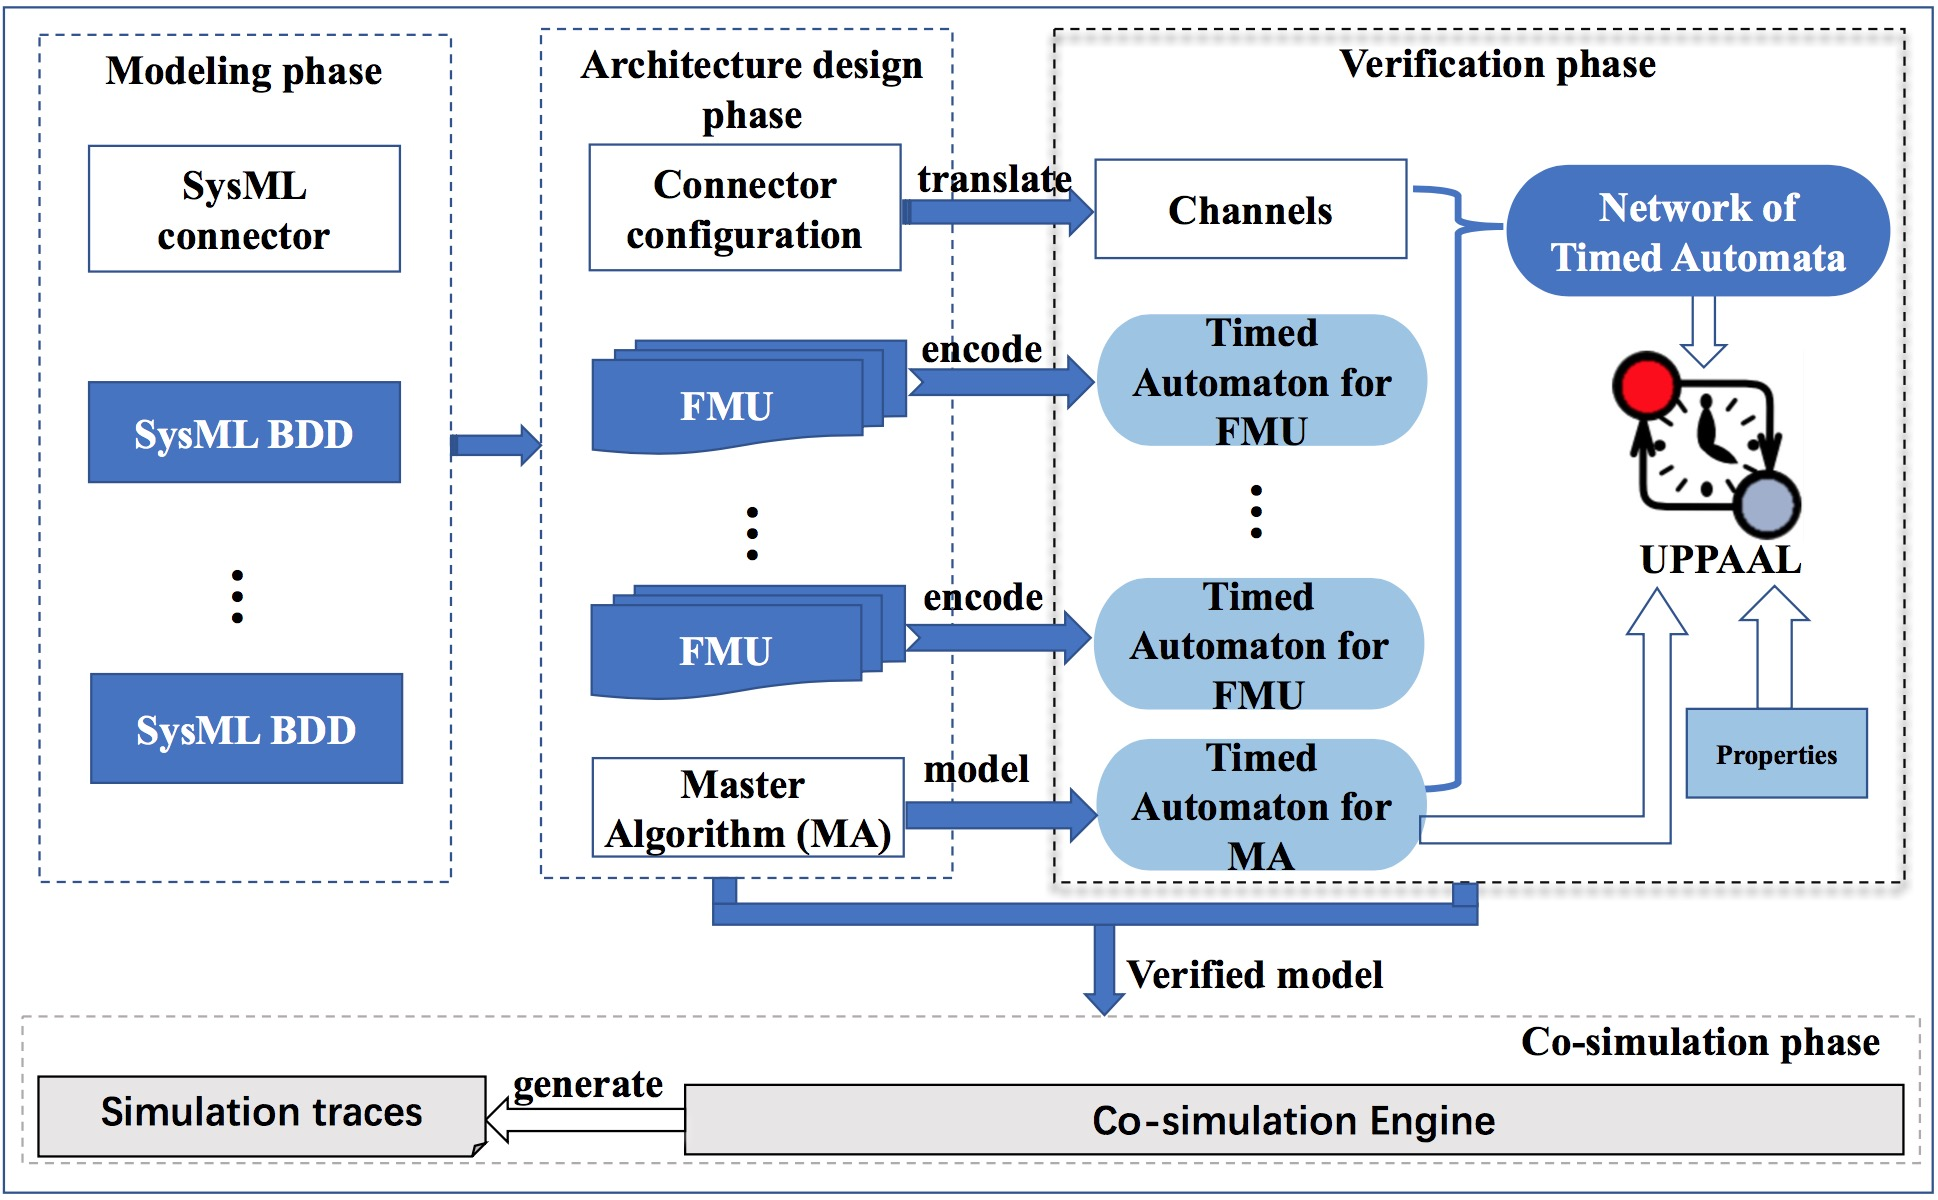
\includegraphics[width=3.5in,height=2.3in]{fig/approachnew.png}}
	\caption{A schematic view of our approach.}
	\label{paper-arc}
\end{figure}

\subsection{Encoding FMUs as TA}
We find that there is a semantic gap between FMUs and TA. The former focuses on the execution sequence of FMU, which specifies the state change process with time elapsing. Essentially, the execution trace of TA is semantic equivalence to the execution sequence of FMU. Naturally, we propose to encode FMU as TA to analyse the behavior of FMU components without exploring its internal structure. 
Given an FMU $F=(S,U,Y,D,s_{0},set,get,doStep)$, we encode the FMU as TA $\textit{A}=(L,l_{0},E,I)$, the congruent relationships between them are as following:
\begin{itemize}
\item
$L$ is a set of finite locations. Note that the state of the transition system $L_{\textit{A}}$ can be seen as the state of $F$, i.e., $(l,v) as rightarrow s$.
\item
The initial state of the transition system $L_{\textit{A}}$ can be seen as the initial state of $F$, i.e., $(l_{0},v_{0}) as s_{0}$. 
\item
Each input variable $u \in U$ ranges over $Act_{i} \cup \{absent\}$.
\item
Each output variable $y \in Y$ ranges over $Act_{o} \cup \{absent\}$.
\item
An input action $e \in Act_{i}$ is such that the function $set$ of $F$ sets the input variable $u$ with a given value. 
\item
An output action $e \in Act_{o}$ indicates that the function $get$ of $F$ gets the output variable $y$. The set of values in the $Act_{i}$ can be seen as $Y$ of $F$.  
\item
The communication between the network of TA is the same as the I/O dependencies information in FMU. $(u,y) \in D$ denotes that output $y$ depend on input $u$. The output actions also depend on the input actions in TA.
\item
For any $e \in Act$ of A, there is a transition $s \xrightarrow{e} s^{\prime}$, which may be found after the function $doStep$ is executing. For instance, if there is a transition $l \xrightarrow{e} l^{\prime}$ in $A$, at the same time $doStep(s,h)$ may be called which indicates that $F$ accepts the time step $h$ and reaches the new state $s^{\prime}$. However, $F$ maybe rejects the time step, if there is a rollback behavior happens, the transition in TA could be an edge $l^{\prime} \xrightarrow{e} l$, which denotes that a location travels to the former location.

\end{itemize}
\begin{figure}[htbp]
	\centering	{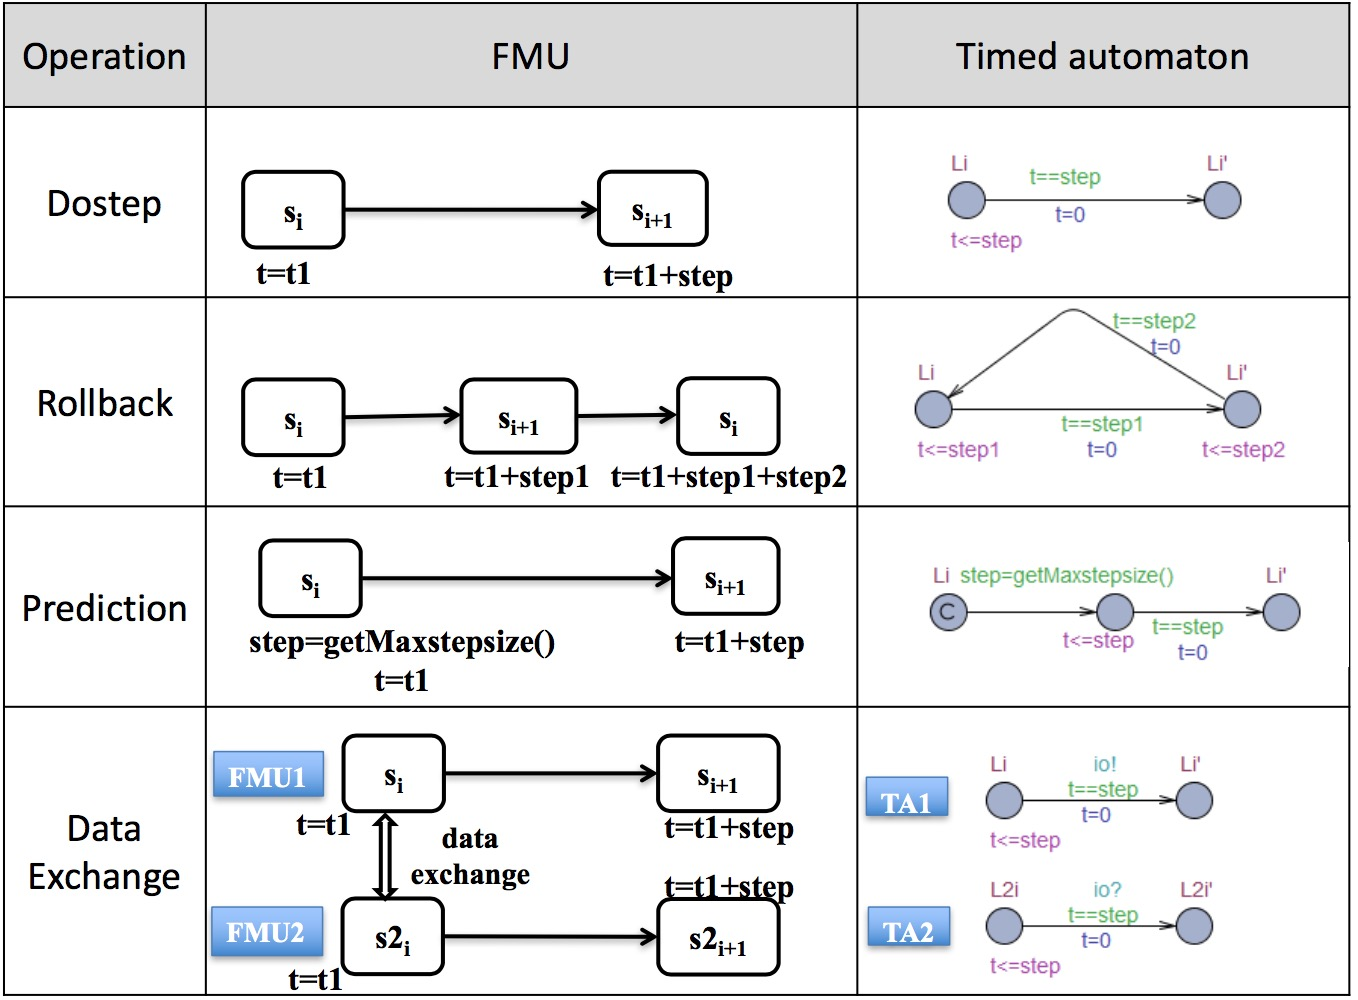
\includegraphics[width=3.5in,height=2.5in]{fig/abstractRole.png}}
	\caption{Encoding rules from FMU as TA.}
	\label{fmutota}
\end{figure}

It is not easy to translate FMU to TA directly. Stavros Tripakis encoding timed automata as FMUs in \cite{Tripakis15}. Inspired by it, we propose some encoding rules according to the congruent relationships. As we can see in the Fig.~\ref{fmutota}, given a state $s_{i}$ at $t_{1}$ in FMU, the operation $Dostep$ makes FMU reach a new state $s_{i+1}$ at $t_{1}+step$. This situation can be encoded as a transition in TA, in which a location $L_{i}$ delays $step$ time and goes to a new location $L_{i}^{\prime}$.

For the operation $Rollback$, given a state $s_{i}$ at $t_{1}$ in FMU, the FMU will do a \emph{step1} to $s_{i+1}$ at $t_{1}+step1$, and then, the operation $rollback$ makes FMU reach the former state $s_{i}$. For this situation, it can be encoded as location $L_{i}$ delays \emph{step1} time units and reach a new location $L_{i}^{\prime}$ after a transition, and then returns to the former location $L_{i}$. 

For the operation $prediction$, given a state $s_{i}$, FMU can get max step size for next step, and then reach a new state $s_{i+1}$ at $t_{1}+step$. For TA, it gets max step size in location $L_{i}$, then it delays $step$ time units and reach a new location $L_{i}^{\prime}$ .

For data exchange between two FMUs in state $s_{i}$ at $t_{1}$, they exchange data at $t_{1}$ and then do the same step to $s_{i+1}$. In TA, there will be a signal \emph{io} to make the two FMUs do the same step from $L_{i}$ to $L_{i+1}$ after data exchange.

Although there are semantic gaps between FMU and TA, we provide appropriate encoding rules to formalism FMUs as TA. It lays the foundation to analyse coordination of CPSs with TA-based model checking. 
%Limited to the length of this paper, we don't prove the correctness of encoding rules. But the encoding process is semantic-preserve. In section \ref{sec:sysml}, we apply these encoding rules to the water tank case study. According to the simulation results, we can find that the encoding rules work well.
As for the correctness of encoding rules, we analyse the equivalence of execution fragment. For the encoding rule of $Dostep$ operation, the execution fragments of FMU and TA are ($s_{i}$, $t_{1}$), ($s_{i+1}$, $t_{1}+step$) and ($l_{i}$, $t$), ($l_{i}^{\prime}$, $t+step$). It means that TA and FMU execute $step$ time units, and jump to a new state or location. For encoding rule of $Rollback$ operation, the execution fragments of FMU and TA are ($s_{i}$, $t_{1}$), ($s_{i+1}$, $t_{1}+step1$), ($s_{i}$, $t_{1}+step1+step2$) and ($l_{i}$, $t$), ($l_{i}^{\prime}$, $t+step1$), ($l_{i}$, $t+step1+step2$). It means that TA and FMU execute $step1$ time units, and jump to a new state or location, and then execute $step2$ time units, return to the previous state or location. For the encoding rule of $Prediction$, the execution fragments of FMU and TA are ($s_{i}$, $t_{1}$), ($s_{i+1}$, $t_{1}+step$) and ($l_{i}$, $t$), ($l_{i}^{\prime}$, $t+step$). For the encoding rule of $Data Exchange$ operation, the execution fragments of FMU1 and TA1 are ($s_{i}$, $t_{1}$), ($s_{i+1}$, $t_{1}+step$) and ($l_{i}$, $t$), ($l_{i}^{\prime}$, $t+step$). The execution fragments of FMU2 and TA2 are ($s2_{i}$, $t_{1}$), ($s2_{i+1}$, $t_{1}+step$) and ($l2_{i}$, $t$), ($l2_{i}^{\prime}$, $t+step$). We have analysed the whole execution trace of FMU and TA for these encoding rules. We find that the execution trace of FMUs and TA are equivalent which means the encoding rules work well. By the analyzing the equivalence of execution trace, the correctness of encoding rules are proved. In section \ref{sec:sysml}, we apply these encoding rules to the water tank system. According to the simulation traces of the case study, we also find that the encoding rules work well.